\documentclass{article}
\usepackage[utf8]{inputenc}

\title{CR_TP2}
\author{philippe.tankmouse }
\date{October 2020}


% New commands declaration

\usepackage[frenchb]{babel}
\usepackage[T1]{fontenc}

\usepackage{natbib,bibentry}
\usepackage{color}
\usepackage{yfonts}
\usepackage{graphicx}
\usepackage{epsfig,subfigure}
\usepackage{amsmath,amssymb,amsfonts}
\usepackage{calc}

\usepackage{array}
\newcolumntype{L}[1]{>{\raggedright\let\newline\\\arraybackslash\hspace{0pt}}m{#1}}
\newcolumntype{C}[1]{>{\centering\let\newline\\\arraybackslash\hspace{0pt}}m{#1}}
\newcolumntype{R}[1]{>{\raggedleft\let\newline\\\arraybackslash\hspace{0pt}}m{#1}}


\DeclareGraphicsExtensions{.eps, .jpg, .png}

\parindent = 0mm

\bibliographystyle{plain}

\hoffset = -20mm
\voffset = -25mm
\textwidth = 160mm
\textheight = 240mm

% \definecolor{lightgray}{gray}{0.2}


\newcommand{\expect}{{\rm I \mkern-2.5mu \nonscript\mkern-.5mu E}}
\newcommand{\equaldef}{\stackrel{d}{=}}
\newcommand{\argmax}{\operatornamewithlimits{argmax}}

\newcommand{\dnu}{16}
\newcommand{\solskip}{10mm}

\renewcommand{\topfraction}{1}
\renewcommand{\bottomfraction}{1}
\renewcommand{\textfraction}{0}

\newcommand{\debutrep}[1]{\color{blue}\begin{center} \hrulefill \textbf{ #1 } \hrulefill \end{center} }
\newcommand{\finrep}{\vspace*{5mm}\hfill $\square$\color{black}\vspace*{5mm}}

\documentclass{article}

\begin{document}

\baselineskip = 4mm
\title{Traitement des Signaux Aléatoires \\
Estimation Spectrale}
\author{\textbf{4 ETI -- CPE Lyon }\\[3mm]
{Travaux Pratiques TSA}}
\date{2020-2021}

\maketitle

\noindent\fbox{
\parbox{\linewidth-2\fboxrule-2\fboxsep}
{ 
\vspace*{2mm}
{\large\bf Noms, Prénoms: }\\[3mm]
{\large\bf Groupe: }\\[3mm]
{\large\bf Date:}\\[2mm]}}
\vspace*{5mm}


\textbf{\Large Objectifs du TP}\\[4mm]

\begin{list}{-}{\setlength{\leftmargin}{3mm} \setlength{\labelwidth}{20mm} \setlength{\labelsep}{2mm} \setlength{\itemsep}{1mm} }
\item Comprendre la notion de densité spectrale d'énergie ou de puissance moyenne
\item Manipuler différents estimateurs empiriques (à partir d'une série temporelle de taille finie) de DSE/DSPM
\item Etudier l'effet du compromis biais-variance d'un estimateur
\end{list}


\vspace*{5mm}

\section{Préparation}

\begin{itemize}
\item[{\bf Question 1}] Comment peut-on calculer simplement la densité spectrale d’énergie (DSE) d’un signal certain d’énergie finie ?

\debutrep{réponse}

\finrep

\item[{\bf Question 2}] Comment est définie la densité spectrale de puissance moyenne (DSPM) d’un processus aléatoire ?

\debutrep{réponse}

\finrep

\item[{\bf Question 3}] Quelles sont les grandeurs qui permettent de chiffrer la qualité d’une estimation dans le cas général ? et la qualité de l’estimation spectrale en particulier.

\debutrep{réponse}

\finrep

\item[{\bf Question 4}] Exprimer la densité spectrale de puissance moyenne (DSPM) GB ( f ) d’un bruit blanc stationnaire centré.

\debutrep{réponse}

\finrep

\item[{\bf Question 5}] Exprimer GX ( f ) , où X(t) est la sortie d’un filtre excité par un bruit blanc centré, en fonction de la DSPM du bruit blanc et des caractéristiques du filtre.

\debutrep{réponse}

\finrep

\item[{\bf Question 6}] En une phrase (sans formule), décrire le procédé de calcul de la DSPM estimée G1 ( f )
d’une séquence aléatoire via l’estimateur simple.

\debutrep{réponse}

\finrep

\item[{\bf Question 7}] Rappeler le mode de graduation d’une TFD-N points en fréquences réduites.

\debutrep{réponse}

\finrep

\item[{\bf Question 8}] Décrire (avec une phrase) le procédé de calcul de la DSPM estimée G2 ( f ) d’une
séquence aléatoire via l’estimateur moyenné.

\debutrep{réponse}

\finrep

\item[{\bf Question 9}] Que signifie le terme «compromis biais-variance» dans le cas de l’estimateur moyenné ?

\debutrep{réponse}

\finrep

\item[{\bf Question 10}] Quelles modifications sont apportées au procédé de calcul de l’estimateur de Welch par rapport à l’estimateur moyenné ?

\debutrep{réponse}

\finrep

\end{itemize}

\clearpage
\setcounter{section}{2}
\section{Estimation de la DSPM d'un bruit blanc gaussien filtré}
\subsection{Génération du bruit à analyser}

A quoi sert l'entier permettant d'initialiser le générateur ?\\

Le problème est qu'il est compliqué d'analyser des processus aléatoire car cela reviendrait à comparer des signaux avec les même caractéristique mais des réalisations différentes. L'option \textit{seed} des fonctions \textit{rnd, rand} sur MATLAB nous permet de fixer la suite de nombre aléatoires dans un ordre précis pour que les n réalisations soit identiques. Ainsi, on étudie un processus pseudo-aléatoire car prédictible.

\subsection{Estimateur spectral simple}
\subsubsection{Script de la fonction {\tt Matlab} développée}

Le code de la focntion \textit{ESS}, il tronqué de sa partie affichage et de ses commentaires pour des raisons de lisibilité mais vous pouvez le retrouver complet en annexes : 
\begin{verbatim}
function  ESS(x,nd,nf,NFFT) ;
    % ---Initialisation des variables ---
    x_seq = x(nd : nf); %Sequence à analyser
    N = nf - nd +1; %Longueur de la sequence
    
    % ---Création de l'estimateur 1 ---
    X = fft(x_seq,NFFT); %Transofrmée N points de la séquence  
    gamma_x_c = ((abs(X)).^2)/N; %Estimation simple
    log_gamma_x_c = 10*log10(gamma_x_c); %Passage au log (forme quadratique donc log * 10)
    
    % ---DSP moyenne vraie et (gamma(f) * Wbm(f))(f)
    [Gth,Gbiais,fth]=sptheo(N,'simple');
    f_abs = 0:1/NFFT:1-1/NFFT;
    
    % ---Partie affichage ---
    figure(2)
    plot(f_abs,log_gamma_x_c,fth,Gth,'k',fth,Gbiais,'r')
    axis([0 0.5 -60 10])
    legend('Estimation de la DSP','DSPMV','Convolution de la DSP et de la fenetre de Barlett')
    title("Etude de l'estimateur simple")
end
\end{verbatim}

\newpage
\subsubsection{Expérimentation}

\begin{enumerate}
\renewcommand{\theenumi}{\Alph{enumi}}
\item Étude du biais et de la variance en fonction du nombre $N$ d'échantillons de bruit

Pour l'étude du biais, nous allons faire varier le paramètre d'entrée N de la fonction \textit{ESS} de 1000 échantillons à 100000 échantillons.

\begin{figure}[h]
\centerline{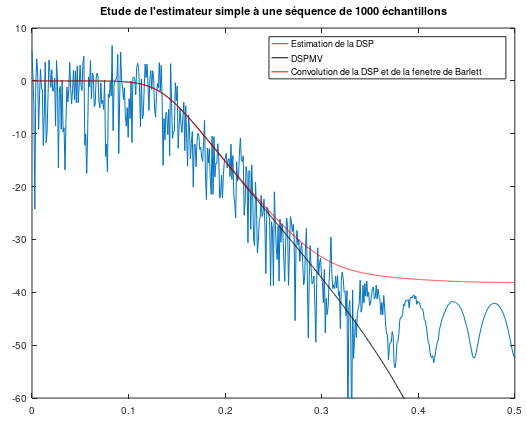
\includegraphics[width=0.52\textwidth]{images/casESN1000.png}}
\caption{$N$ faible (1000)-- indice de début de la séquence à 1}
\end{figure}

\begin{figure}[h]
\centerline{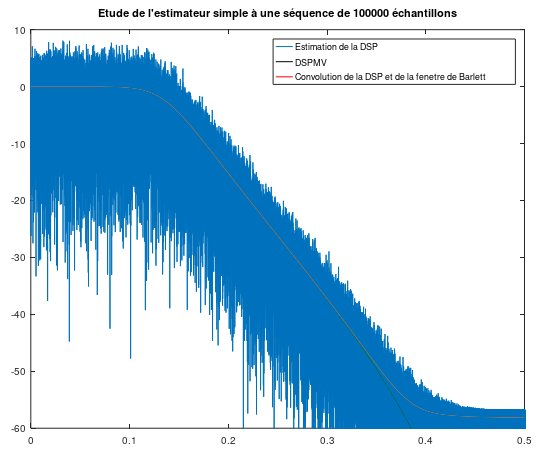
\includegraphics[width=0.52\textwidth]{images/casESN100000.png}}
\caption{$N$ élevé (100 000)-- indice de début de la séquence à 1}
\end{figure}

Sur les figures 1 et 2, nous pouvons observer 3 courbes, la bleu correspond à la densité spectrale obtenues à partir d'une séquence empirique à $N$ points. La courbe noire correspond à la densité spectrale théorique non biaisée et la rouge correspond à la densité spectrale convolué par une fenêtre de BARLETT (donc biaisé). 
Ainsi, nous pouvons constater que si N est faible alors la DS empirique correspond à l'estimateur non-biaisé sur les basses-fréquences mais va être biasié sur les hautes fréquences et une variance qui est "faible" sur toutes la DSP.
Inversement, avec un N important le biais va être "faible" car la courbe bleu suit la DST mais la variance est très importantes. \\
Nous pouvons expliquer ce comportement à l'aide du phénomène de convolution par la fenêtre de BARRET car plus on a une fenêtre tend vers l'inifinie (plus physiquement le signale est long dans le temps) et plus le replie temporelle va être faible donc les hautes fréquences de la DST ne vont pas être impactées par les basses fréquences et le biais diminues. Le problème est que la variance est obtenues à l'aide de la relation :\\
\centerline{$VAR(ES) = \Gamma^2(x) + [1+(sin(2*pi*f*N)/(N*2*pi*f))^2]$}
 
\newline

\item Etude du biais et de la variance en fonction de la réalisation considérée, à $N$ fixé 
\newline
Pour cette étude, nous avons fixé taille du N à 1000 échantillons et l'on obtient les figures suivantes : 

\begin{figure}[h]

\centerline{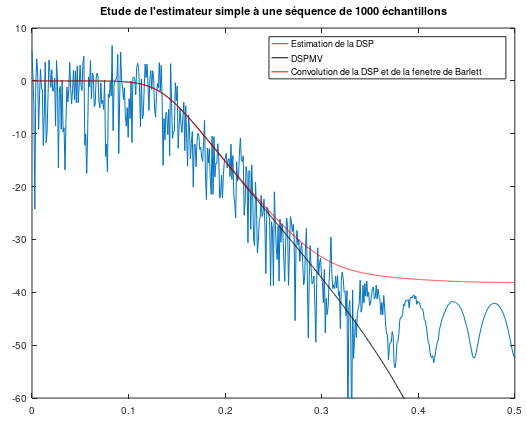
\includegraphics[width=0.55\textwidth]{images/casESN1000.png}}
\caption{$N \sim 1000$ -- indice de début de la séquence à 1}
\end{figure}

\begin{figure}[h]

\centerline{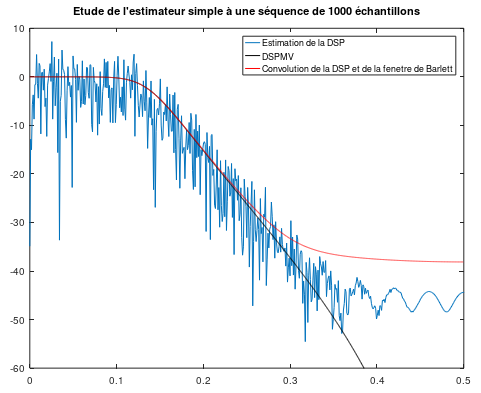
\includegraphics[width=0.55\textwidth]{images/casESN1000PD2000.PNG}}
\caption{$N \sim 1000$  -- indice de début de la séquence fixé à une autre position ($\gg 1000$) dans la séquence}
\end{figure}

Nous pouvons observer que sur les figure 3 et 4 (pour une séquence qui débute à 2000), les courbes obtenues sont semblables. Ce résultat est cohérent car le signal  observé est un bruit blanc Gaussien qui à comme propriété d'être stationnaire donc l'intervalle d'échantillons peut être quelconque car n'influe pas sur l'étude, tant que l'on conserve une même taille $N$. 
\newline

\clearpage
\item Etude du biais et de la variance en fonction du nombre $NFFT$ de FFT
\newline
Pour cette étude, nous avons fixé taille du N à 1000 échantillons et l'on obtient les figures suivantes : 
\begin{figure}[h]
\centerline{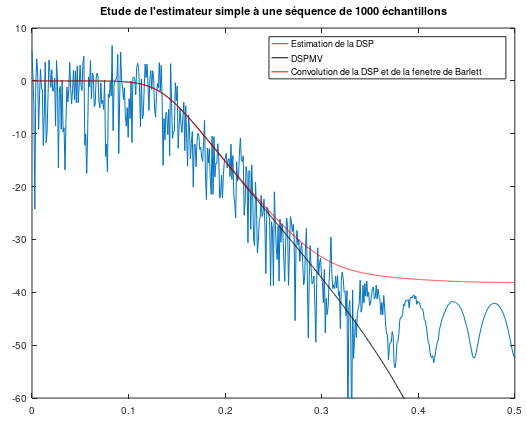
\includegraphics[width=0.55\textwidth]{images/casESN1000.png}}
\caption{$N$ constant -- indice de début de la séquence à 1 -- $NFFT \sim N$}
\end{figure}

\begin{figure}[h]
\centerline{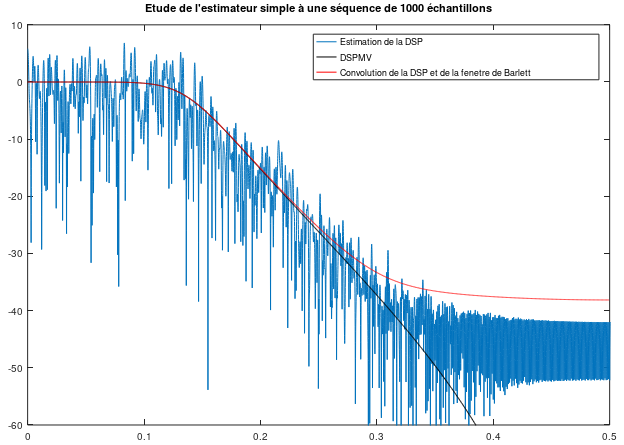
\includegraphics[width=0.55\textwidth]{images/casESN1000FFT214.png}}
\caption{$N$ constant -- indice de début de la séquence à 1 -- $NFFT (2**14) \gg N$}
\end{figure}

Nous pouvons observer que sur les figure 5 et 6 (une FFT sur $2^14$ points), les courbes obtenues sont semblables. Ce résultat est cohérent car pour obtenir les densités spectrales le paramètre $NFFT$ n'influence que le nombre de points pour la Transformé de Fourier à N points. Et va permettre d'augmenter la précisions de la courbe.  Ainsi il ne peut pas influé sur l'étude, tant que l'on prend $NFFT > N$. 
\newline

\item Conclusion
Quel est le principal défaut de l'estimateur simple ?\\
\newline
A l'aide de l'étude réalisé, nous pouvons conclure que l'estimateur simple à comme principale défaut sa variance car N est grand est plus le terme carré pour obtenir la variance va "exploser" et cela devient compliqué d'analyser la courbe. Ainsi cette estimateur n'est pas de bonne qualité.  

\end{enumerate}

\clearpage
\subsection{Estimateur spectral moyenné}

\textbf{On fixera $\mathbf{N=4096}$ dans tout ce qui suit.}

\subsubsection{Script de la fonction {\tt Matlab} développé}

\debutrep{code ci-dessous}
\begin{verbatim}

\end{verbatim}
\finrep


\subsubsection{Expérimentation}

En précisant bien la valeur des paramètres utilisés pour les essais, affichez les figures correspondantes aux conditions indiquées.
\debutrep{figure ci-dessous}

\begin{figure}[h]

\caption{$N=4096$ -- tranches courtes $M = ??? $, $NFFT = ???$}
\end{figure}
\finrep

Commentaires
\debutrep{réponse ci-dessous}

\finrep

\debutrep{figure ci-dessous}
\begin{figure}[h]

\caption{$N=4096$ -- tranches longues $M = ???$, $NFFT = ???$}
\end{figure}

\finrep

Commentaires
\debutrep{réponse ci-dessous}

\finrep

\debutrep{figure ci-dessous}
\begin{figure}[h]

\caption{$N=4096$ -- \og Meilleur \fg compromis biais variance atteint pour $M = ???$, $NFFT = ???$}
\end{figure}

\finrep

Quelle information permettrait d'obtenir le meilleur compromis biais-variance? 

\debutrep{réponse ci-dessous}

\finrep

\clearpage
\section{Estimateur de Welch}

\subsection{Etude préalable des fenêtres}

Quelles différences de comportement fréquentiel peut-on observer pour les 6 fenêtres proposées (lobe principal, lobes latéraux\ldots).

\subsubsection{Script de la fonction {\tt Matlab} développée}

\debutrep{code ci-dessous}
\begin{verbatim}

\end{verbatim}
\finrep

\subsubsection{Expérimentation}

\begin{enumerate}
\renewcommand{\theenumi}{\Alph{enumi}}

\item Etude du biais et de la variance en fonction du taux de recouvrement entre tranches

Pour $N$, $M$ et $NFFT$ fixés et pour une  fenêtre choisie,  tracez les figures correspondantes aux conditions indiquées ci-dessous.

\debutrep{figure ci-dessous}
\begin{figure}[h]

\caption{$N = 4096$ -- $M = ???$, $NFFT = ???$. Choix de fenêtre = ??? -- Recouvrement de $0\%$}
\end{figure}

\begin{figure}[h]

\caption{$N = 4096$ -- $M = ???$, $NFFT = ???$. Choix de fenêtre = ??? -- Recouvrement de $50\%$}
\end{figure}

\finrep

Que permet le recouvrement entre tranches ?

\debutrep{réponse ci-dessous}

\finrep

\item Etude du biais et de la variance en fonction de la fenêtre utilisée

Pour $N$, $M$ et $NFFT$ fixés et pour différents choix de fenêtre,  tracez les figures correspondantes aux conditions indiquées ci-dessous.

\debutrep{figure ci-dessous}
\begin{figure}[h]

\caption{$N = 4096$ -- $M = ???$, $NFFT = ???$. Fenêtre Rectangle -- Recouvrement de $50\%$}
\end{figure}

\begin{figure}[h]

\caption{$N = 4096$ -- $M = ???$, $NFFT = ???$. Fenêtre ??? -- Recouvrement de $50\%$}
\end{figure}

\finrep

Que permet l'utilisation d'une fenêtre autre que rectangulaire ? Expliquer.

\debutrep{réponse ci-dessous}

\finrep

\end{enumerate}

Pour quelles valeurs des paramètres d'analyse obtenez vous le \og meilleur \fg résultat (celui qui vous parait le plus satisfaisant)?

\debutrep{réponse ci-dessous}

Longueur de la séquence analysée $N = ???$ \\
Longueur des tranches $M = ???$ \\
Type de fenêtre ??? \\
Taux de recouvrement = ??? \\
Nombre de points de transformée de Fourier $NFFT = ???$

\finrep

\section{Utilisation des estimateurs précédents pour analyser un signal inconnu}

\subsection{Modification des programmes}

Script d'une des fonctions modifiée
\newline
\newline
Les fonctions ont étés modifiées en retirant la partie création de la partie théorique car le signal étudié n'est plus un bruit blanc mais un signal inconnu et fournie sur CPe-campus.
\newline
L'autre modification est que nous avons ajouté des paramètres de retours et retirer la partie affichage interne à chaque fonction. Ainsi, nous avons centralisé l'affichage dans le code main et utilisé la fonction \textit{semilogy} pour obtenir une étude plus ergonomique. 
Ci-dessous le code de la fonction \textit{ESS.c }, l'estimateur Simple. Tous les codes avec leurs commentaires sont disponibles en Annexes. 

\begin{verbatim}
function [gamma_x_c,f_abs] = ESS(x,nd,nf,NFFT) ;
    % ---Initialisation des variables ---
    x_seq = x(nd : nf); %Sequence à  analyser
    N = nf - nd +1; %Longueur de la sequence
    
    % ---Création de l'estimateur 1 ---
    X = fft(x_seq,NFFT); %Transofrmée N points de la séquence  
    gamma_x_c = ((abs(X)).^2)/N; %Estimation simple
    f_abs = 0 : 1/NFFT: 1-1/NFFT;
end

\end{verbatim}


\subsection{Expérimentation}

Afficher les spectres estimés obtenus avec chacune des 3 méthodes étudiées.


\begin{figure}[h]
\centerline{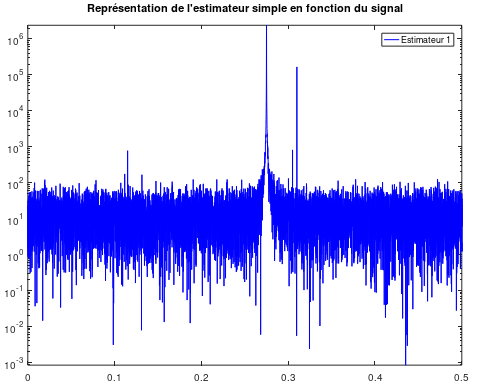
\includegraphics[width=0.52\textwidth]{images/casESSimpleSignalInconnue.png}}
\caption{Estimateur spectral simple. \textit{Les paramètres sont un N de 100000 (totalité du signal) et un NFFT de 16384 points}.}
\end{figure}

\begin{figure}[h]
\centerline{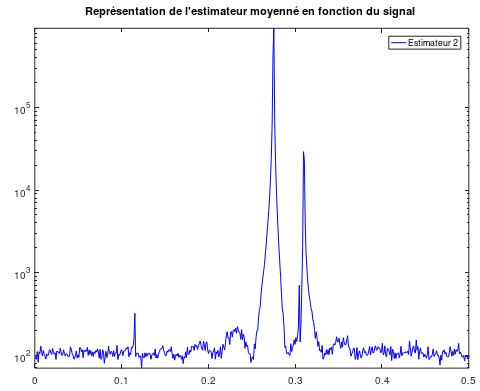
\includegraphics[width=0.52\textwidth]{images/casESMSignalInconnue.png}}
\caption{Estimateur spectral Moyenné. \textit{Les paramètres sont un M de 1000 et une NFFT de 1024 points}.}
\end{figure}

\begin{figure}[h]
\centerline{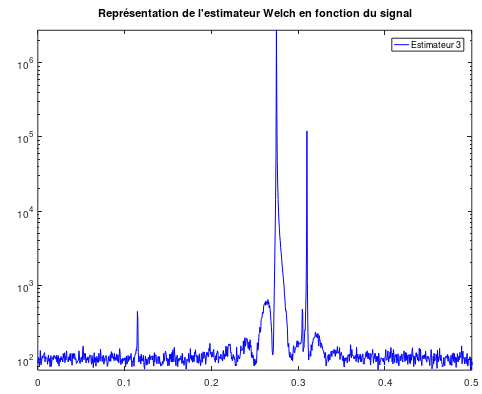
\includegraphics[width=0.52\textwidth]{images/casESWSignalInconnue.png}}
\caption{Estimateur spectral de Welch. \textit{Les paramètres sont un M de 2000 et une NFFT de 2048 points et de 50\% d\'Overlap}.}
\end{figure}

\finrep
\newpage
Décrivez précisément la démarche expérimentale suivie. Avec quelle méthode êtes vous capable avec certitude de décrire le contenu fréquentiel de ce signal ?\newline

Dans un premier temps, nous utilisons l'estimateur simple car bien qu'en partie 1, nous avons conclue qu'il est peu fiable au niveau du biais-variance, l'étude ne prennais pas en compte les propriétés de résolution fréquentielle. Or dans son cas, la formule est : $ Rfrequ = 1.28/2N $ or pour un N de 10000 nous obtenons une résolution précise et nous pouvons étudier facilement les éléments qui compose le spectre. \newline
Cette première étude va permettre d'ajuster les paramètres des Estimateur Moyenné et de Welch, nous savons que la résolution fréquentielle est obtenu à l'aide de : $ Rfrequ = 1.28/2M $ or avec la première étude, il est apparus que deux composantes sont proches donc la taille de la fenêtre devra être grande pour obtenir une résolution fréquentielle suffisante.\newline
Dans notre cas, empiriquement nous avons choisie une fenêtre d'une taille de 1000 et une transformée de Fourier de 1024 points. \newline
Le soucis est que cette configuration ne fonctionne pas dans le cadre de l'estimateur Welch car sinon la Densité Spectrale "perd" une composante car elle est "absorbée" par une autre. Ainsi, nous somme contrains de doublé la taille de la fenêtre M.

\subsubsection{Interprétations}

\begin{enumerate}
\renewcommand{\theenumi}{\Alph{enumi}}

\item Que inconvénient majeur l'utilisation d'une fenêtre (d'apodisation en temps) engendre-t-elle?
L'inconvénient majeur d'une telle méthode est que l'on va biasié notre estimateur par une convolution de sa transformée de Fourier. Et cette estimateur devient très variable car une partie son biais va dépendre du type de la fenêtre employé. \newline
C'est pour cela qu'il est recommandé une fenêtre qui a une transformée de Fourier proche du Dirac car cela facilite l'étude de la convvolution.

\item Décrire (sans dessin) la forme de la DSPM obtenue.
La DSPM se compose de 4 éléments qui sont similaires à des pics de Diracs et  aux fréquence réduite suivante (il s'agit de constatation graphique et donc imprécise) : 
\begin{center}
\begin{enumerate}
    \item f1 = 0.12
    \item f2 = 0.27
    \item f3 = 0.31 
    \item f4 = 0.33
\end{enumerate}
\end{center}

\item Quelles informations la forme de cette DSPM apporte-t-elle sur le contenu (la nature) du signal?
\newline
Si l'on fait l'hypothèse que les Pics observés sont des Diracs alors à l'aide des propriétés de la transformée de Fourier, nous pouvons en déduire que ce signal inconnue correspond à la somme de 4 sinus avec des amplitudes et phases différentes.

\item Quelles mesures concernant  les caractéristiques du signal peut-on effectuer sur la DSPM?
Les caractéristiques remarquable du signal sont les fréquences de ses composantes sur sa DSPM et les valeurs d'amplitudes des dites composantes.
\end{enumerate}

\section{Annexes}
\subsection{Fonction de la Partie 1 : }
\subsubsection{Fonction de l'Estimateur Simple }
\begin{verbatim}
function  ESS(x,nd,nf,NFFT) ;
    %Input : 
    % x - séquence brut 
    %nd - premier indice de la séquence à  analyser
    %nf - dernier indice de la séquence à  analyser
    %NFFT - nombre de points de TFD-N points
    %Output : 
    %None
    
    % ---Initialisation des variables ---
    x_seq = x(nd : nf); %Sequence à analyser
    N = nf - nd +1; %Longueur de la sequence
    
    % ---Création de l'estimateur 1 ---
    X = fft(x_seq,NFFT); %Transofrmée N points de la séquence  
    gamma_x_c = ((abs(X)).^2)/N; %Estimation simple
    log_gamma_x_c = 10*log10(gamma_x_c); %Passage au log (forme quadratique donc log * 10)
    
    % ---DSP moyenne vraie et (gamma(f) * Wbm(f))(f)
    [Gth,Gbiais,fth]=sptheo(N,'simple');
    f_abs = 0:1/NFFT:1-1/NFFT;
    
    % ---Partie affichage ---
    figure(2)
    plot(f_abs,log_gamma_x_c,fth,Gth,'k',fth,Gbiais,'r')
    axis([0 0.5 -60 10])
    legend('Estimation de la DSP','DSPMV','Convolution de la DSP et de la fenetre de Barlett')
    title(["Etude de l'estimateur simple à une séquence de ",int2str(N)," échantillons"])
end
\end{verbatim}
\newpage
\subsubsection{Fonction de l'Estimateur Moyenné }
\begin{verbatim}
%% Code à saisir 
\end{verbatim}
\newpage
\subsubsection{Fonction de l'Estimateur de Welch }
\begin{verbatim}
%% code à saisir
\end{verbatim}
\newpage
\subsubsection{Code Main }
\begin{verbatim}
% ----
%  Auteur : Philippe CHARRAT & Axel BRUYERE
%  TP 2 - T.S.A : Estimateurs
%  But : Partie 2
% ----
clc;clear variables;close all;

% Génération d'un bruit blanc --- 
s = genbrfil; % Fonction fournie sur Cpe-campus

% génération des différents estimateurs
ESS(s,1,1000,2^14);
ESM(s,10000,500,512);
ESW(s,10000,'rectwin',500,250,512);


\end{verbatim}
\newpage
\subsection{Fonction de la Partie 2 : }
\subsubsection{Fonction de l'Estimateur Simple }
\begin{verbatim}
function [gamma_x_c,f_abs] = ESS(x,nd,nf,NFFT) ;
    %Inputs : 
    % x - séquence brut 
    %nd - premier indice de la séquence à  analyser
    %nf - dernier indice de la séquence à  analyser
    %NFFT - nombre de points de TFD-N points
    %
    %Outputs : 
    %gamma_x_c = vecteur contenant la DS pour l'estimateur 1 
    %fabs = vecteur d'abscisses 
    
    % ---Initialisation des variables ---
    x_seq = x(nd : nf); %Sequence à  analyser
    N = nf - nd +1; %Longueur de la sequence
    
    % ---Création de l'estimateur 1 ---
    X = fft(x_seq,NFFT); %Transofrmée N points de la séquence  
    gamma_x_c = ((abs(X)).^2)/N; %Estimation simple
    f_abs = 0 : 1/NFFT: 1-1/NFFT;

end
\end{verbatim}
\newpage
\subsubsection{Fonction de l'Estimateur Moyenné }
\begin{verbatim}
function [gamma_xd_c,fabs] = ESM2(x,N,M,nfft)
    % Inputs :
    % x - séquence brut 
    % N - nombre d'échantillons maximum
    % M - nombre d'échantillons d'une sous fenêtre 
    % nfft - nombre de points fft à N points
    % 
    % Oututs :
    % none 
    
    % Initialisation des variables ---
    x_seq = x(1 : N); %sequence à analyser
    fenetre = rectwin(M); % Fenetre taille M << N
    noverlap = 0; % Chevauchement 
    
    % Création de l'estimateur 2 ---
    [gamma_xd_c,fabs] = pwelch(x_seq,fenetre,noverlap,nfft,1,'twosided');
end
\end{verbatim}
\newpage
\subsubsection{Fonction de l'Estimateur de Welch }
\begin{verbatim}
function [gamma_x_c,f_abs] = ESW2(x,N,fenetre_char,M,NOVERLAP,NFFT)
    %Inputs : 
    % x - séquence brut 
    %nd - premier indice de la séquence à  analyser
    %nf - dernier indice de la séquence à  analyser
    %NFFT - nombre de points de TFD-N points
    %fenetre_char : str contenant le type de la fenêtre
    %Noverlap : la couvertures entre les différentes fenêtre en % 
    %
    %Outputs : 
    %gamma_x_c = vecteur contenant la DS pour l'estimateur 3 
    %fabs = vecteur d'abscisses 
    % ---Initialisation des variables ---
    x_seq = x(1:N);
    eval(['WIN=',fenetre_char,'(M)']);
    f_abs = 0:1/NFFT:1-1/NFFT;
    
% ---Création de l'estimateur 3---
    [gamma_x_c,fabs] = pwelch(x_seq,WIN,NOVERLAP,NFFT,1,'twosided');  
end
\end{verbatim}
\newpage
\subsubsection{Code Main }
\begin{verbatim}
% ----
%  Auteur : Philippe CHARRAT & Axel BRUYERE
%  TP 1 - T.S.A : Estimateurs
%  But : Partie 2
% ----
clc;
clear variables;
close all;

% Partie Initialisation des différents estimateurs
load('../sig.mat');
[gamma_x_e1,fabs1] =ESS2(s,1,100000,2^14);
[gamma_x_e2,fabs2] =ESM2(s,100000,1000,1024);
[gamma_x_e3,fabs3] =ESW2(s,100000,'rectwin',2000,0.5,2048);
    
% Partie affichage ---
figure(1);
subplot(3,1,1)
semilogy(fabs1,gamma_x_e1,'b');
axis([0 0.5 -inf inf])
legend('Estimateur 1')
title("Représentation de l'estimateur simple en fonction du signal")

subplot(3,1,2)
semilogy(fabs2,gamma_x_e2,'b');
axis([0 0.5 -inf inf])
legend('Estimateur 2')
title("Représentation de l'estimateur moyenné en fonction du signal ")

subplot(3,1,3)
semilogy(fabs3,gamma_x_e3,'b');
axis([0 0.5 -inf inf])
legend('Estimateur 3')
title("Représentation de l'estimateur Welch en fonction du signal")
\end{verbatim}
\newpage
\subsection{Figures de la Partie 1 : }
\subsubsection{Figures de l'Estimateur Simple : cas à 1000 points}
\begin{figure}[h]
\centerline{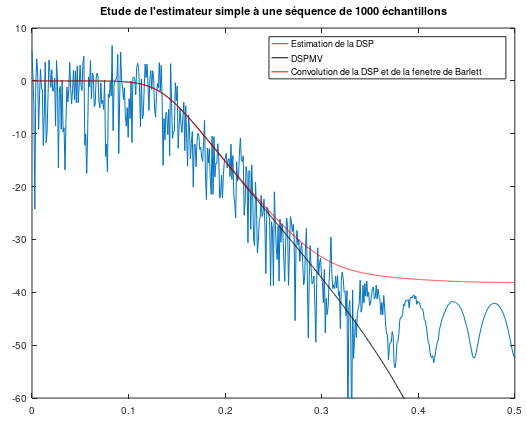
\includegraphics[width=1\textwidth]{images/casESN1000.png}}
\caption{Cas de N = 1000 points}
\end{figure}
\newpage
\subsubsection{Figures de l'Estimateur Simple : cas à 10000 points}
\begin{figure}[h]
\centerline{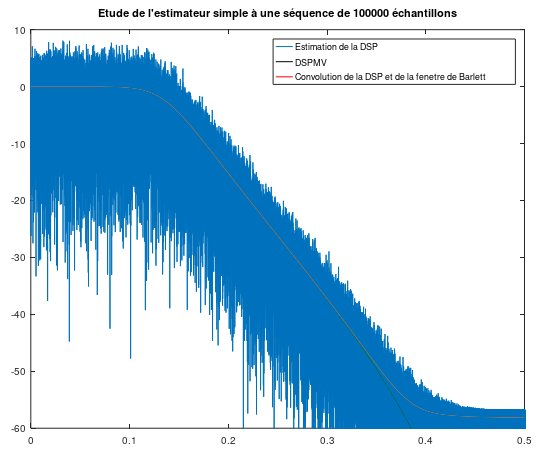
\includegraphics[width=1\textwidth]{images/casESN100000.png}}
\caption{Cas N = 10000 points }
\end{figure}
\newpage
\subsubsection{Figures de l'Estimateur Simple : cas pour  NFFT >> N}
\begin{figure}[h]
\centerline{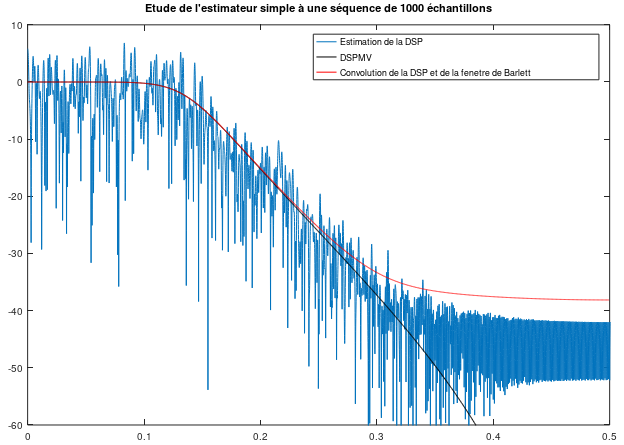
\includegraphics[width=1\textwidth]{images/casESN1000FFT214.png}}
\caption{Cas N = 1000 et NFFT = 2\^14 points}
\end{figure}
\newpage
\subsubsection{Figures de l'Estimateur Simple : cas pour Ndébut >> 1}
\begin{figure}[h]
\centerline{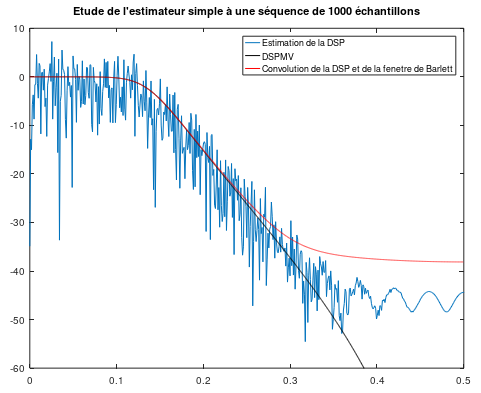
\includegraphics[width=1\textwidth]{images/casESN1000PD2000.PNG}}
\caption{Cas N = 1000 et indice de début est 2000}
\end{figure}
\newpage
\subsection{Figures de la Partie 2 : }
\subsubsection{Figures général}
\begin{figure}[h]
\centerline{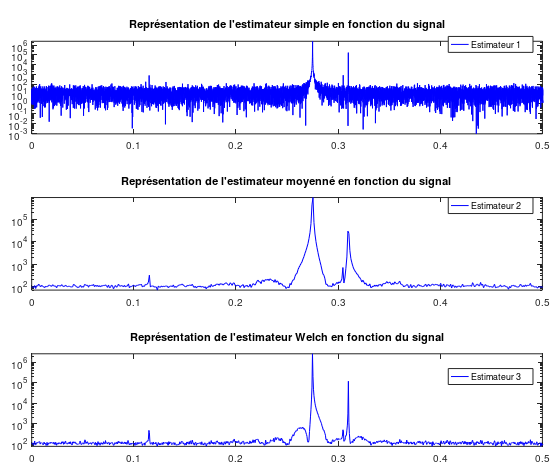
\includegraphics[width=1\textwidth]{images/casgenpartie2.png}}
\caption{Cas Général}
\end{figure}
\newpage
\subsubsection{Figures de l'Estimateur Simple}
\begin{figure}[h]
\centerline{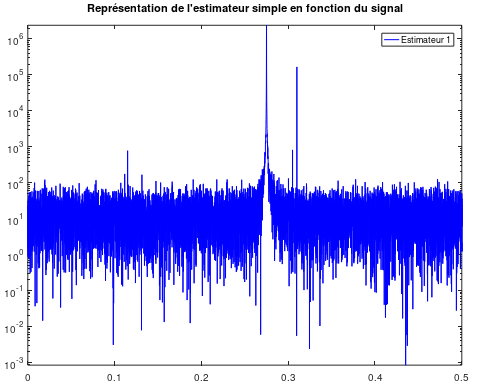
\includegraphics[width=1\textwidth]{images/casESSimpleSignalInconnue.png}}
\caption{Cas pour l'estimateur simple}
\end{figure}
\newpage
\subsubsection{Figures de l'Estimateur Moyenné}
\begin{figure}[h]
\centerline{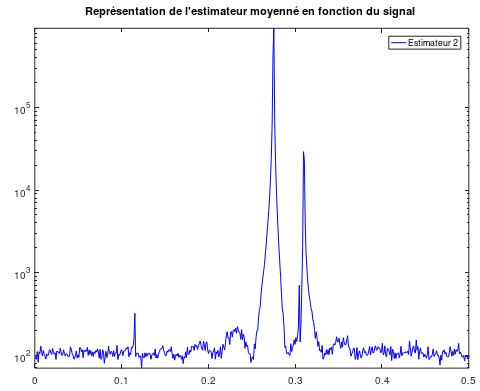
\includegraphics[width=1\textwidth]{images/casESMSignalInconnue.png}}
\caption{Cas pour l'estimateur moyenné}
\end{figure}
\newpage
\subsubsection{Figures de l'Estimateur de Welch}
\begin{figure}[h]
\centerline{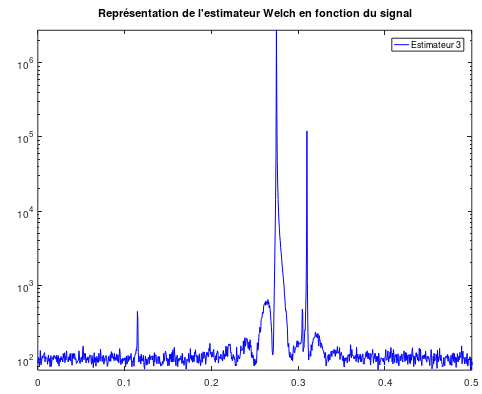
\includegraphics[width=1\textwidth]{images/casESWSignalInconnue.png}}
\caption{Cas pour l'estimateur de Welch}
\end{figure}

\end{document}